\chapter{ПРЕДЛОЖЕННЫЙ ПОДХОД}
\label{ch:ПРЕДЛОЖЕННЫЙ ПОДХОД}

В этой главе будет дано описание концептуальной модели предложенного подхода. В первых секциях описаны базовая схема работы и архитектура системы. В последующих секциях представлены детали используемых методов для обработки входных данных и аппроксимации траекторий, схематично изложены основные алгоритмы.

\section{Концептуальная модель фреймворка}
\label{ch:Концептуальная модель фреймворка}

Основной целью данной работы является анализ пространственно-временных данных о траекториях движущихся ТС, полученных с камер видеонаблюдения, и решение задачи определения аномалий. Для решения поставленной задачи подход, основанный на кластеризации, был выбран как основа: сначала входные траектории используются как обучающие данные для определения кластеров и их моделирования; кластеры классифицируются как нормальные или аномальные в зависимости от количества траекторий в кластере; затем классификатор помечает входную траекторию как нормальную или аномальную на основании обученной модели кластеров.

Основной вклад этой работы заключается в попытке минимизировать проблему, связанную с неопределенностью данных, и повысить точность результатов путем использования адаптивных параметров при подсчете схожести траекторий: в новом подходе будет учитываться позиция движущегося объекта по отношению к камере. Для этих целей был разработан фреймворк, решающий задачи определения частых траекторий движения и обнаружения аномальных.

Основной рабочий процесс фреймворка состоит из следующих этапов (Figure \ref{fig:flowchart}):
\begin{itemize}
	\item обработка входных данных и парсинг траекторий,
	\item фильтрация траекторий на основании количества точек траектории и итогового пройденного расстояния,
	\item аппроксимация траекторий с использованием полиномиальной регрессии,
	\item подсчет схожести траекторий и заполнение ``матрицы подобия'',
	\item кластеризация траекторий,
	\item определение нормальных и аномальных кластеров, визуализация кластеров,
	\item моделирование нормальных кластеров
	\item классификация входной траектории как нормальной или аномальной.
\end{itemize}

\begin{figure}[!htb]
	\centering{}
	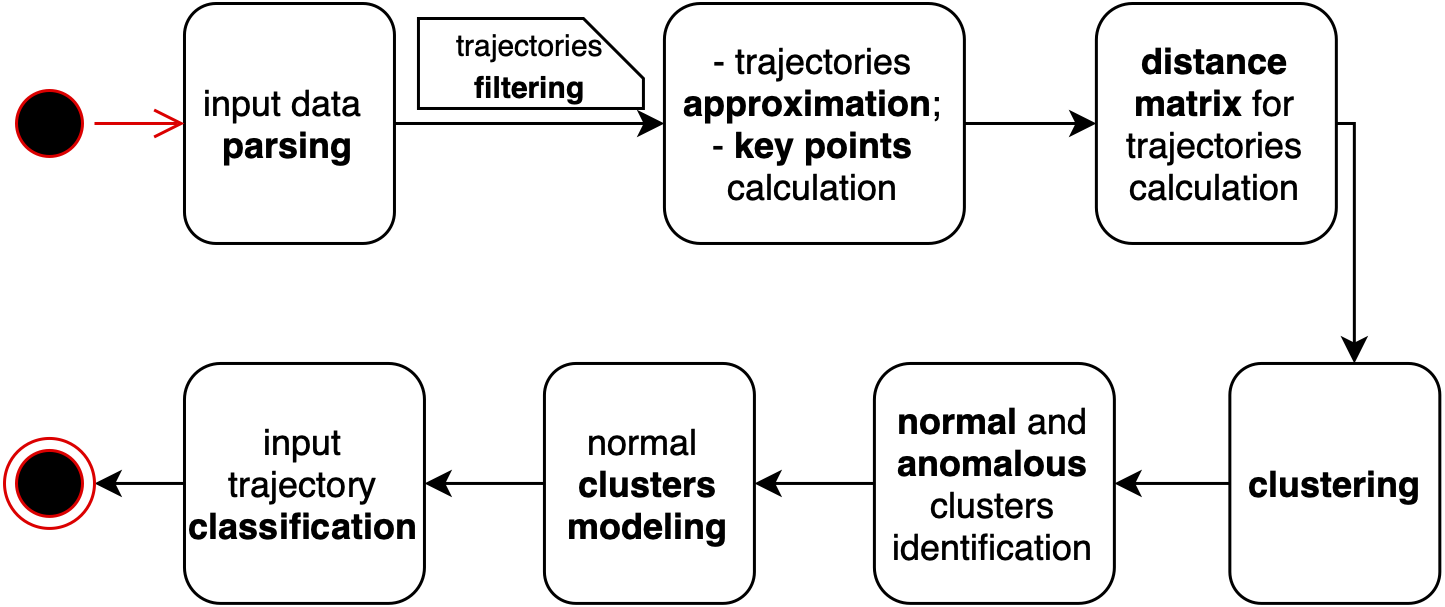
\includegraphics[width=0.8\textwidth]{images/flowchart.png}
	\caption{Основные этапы работы фреймворка}
	\label{fig:flowchart}
\end{figure}

\section{Архитектура фреймворка}

Архитектура предложенного подхода основана на работе \cite{inproceedings:7_related_work}, подробно описанной ранее, и состоит из двух частей (\ref{fig:str}):

\begin{itemize}
	\item \textit{offline} -- кластеризация и определние паттернов наиболее часто встречающихся траекторий, и
	\item \textit{online} -- классификация новой траектории как нормальной или аномальной.
\end{itemize}

\begin{figure}[!htb]
	\centering{}
	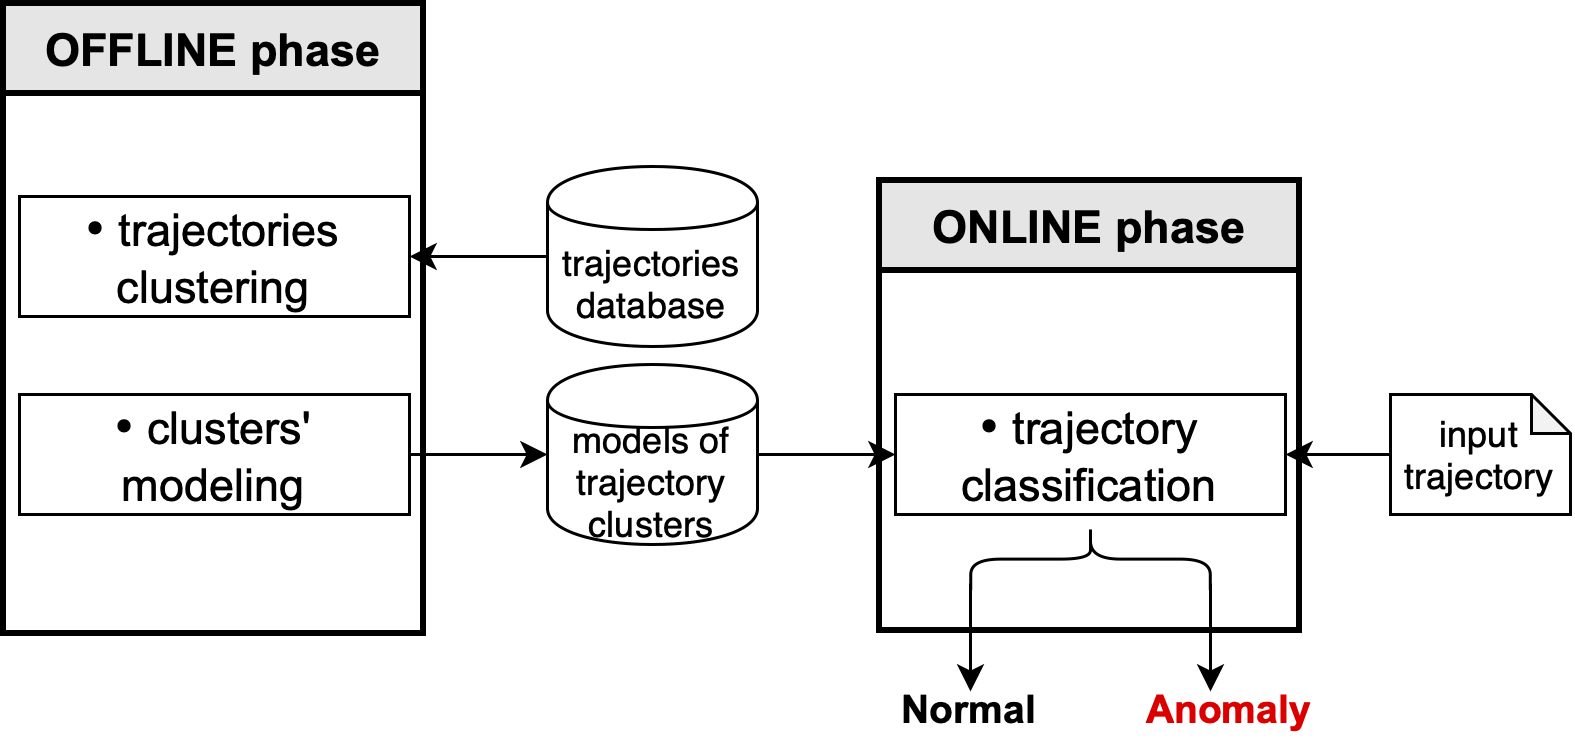
\includegraphics[width=0.8\textwidth]{images/str.png}
	\caption{Схема двухэтапного предложенного подхода}
	\label{fig:str}
\end{figure}

Фреймворк состоит из нескольких модулей, каждый из которых отвечает за выполнение одной из задач из вышеперечисленных этапов рабочего процесса (Figure \ref{fig:proj-arch}):
\begin{itemize}
	\item \textit{entity} -- содержит классы-сущности для хранения таких объектов, как $Trajectory$, $TrajectoryPoint$, $Cluster$ и др.;
	\item \textit{parsing} -- отвечает за парсинг входных данных: считывает данные из 'txt'-файла и создает объекты $TrajectoryPoint$ и $Trajectory$;
	\item \textit{csv} -- изолирует логику работы с 'csv'-файлами, содержит методы чтения и записи, которые используются сначала для сохранения подсчитанных LCSS метрик, а затем для их подгрузки для дальнейшей кластеризации;
	\item \textit{approximation} -- содержит реализацию аппроксимации траекторий методом полиномиальной регрессии и необходимые сопутствующие классы, такие как класс $Polynomial$, расширяющий функционал стандартного $PolynomialFunction$ из библиотеки Apache Math, и др.;
	\item \textit{visualization} -- отвечает за визаулизацию и сохранение полученных результатов, содержит методы для чтения, изменения, сохранения объектов класса $BufferedImage$;
	\item \textit{clustering} -- состоит из класса $Clustering$, который содержит методы для подсчета значений LCSS метрики, кластеризации объектов класса $Trajectory$ и создания объектов класса $Cluster$;
	\item \textit{exception} -- содержит исключения, которые теоретически могут быть выброшены в ходе работы фреймворка (например, $TrajectoryParserException$);
	\item \textit{misc} -- содержит вспомогательные утилитные классы для хранения константных значений и базовых методов, общих для всех модулей разрабатываемой системы.
\end{itemize}

\begin{figure}[!htb]
	\centering{}
	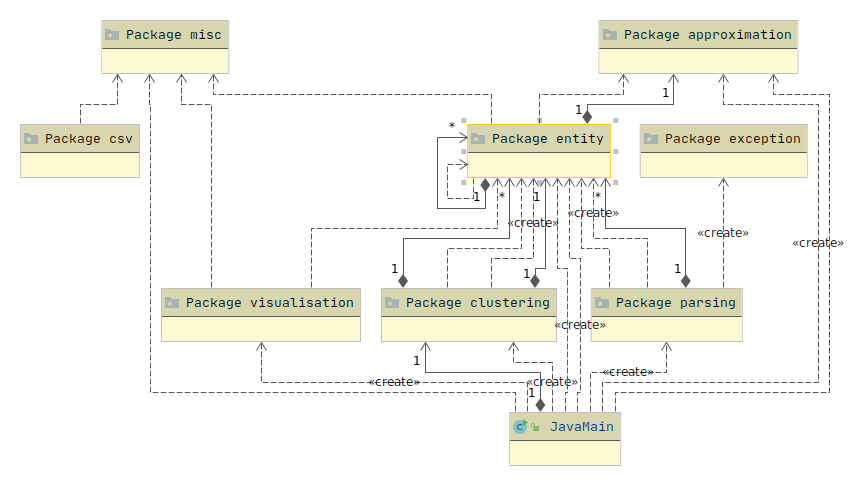
\includegraphics[width=0.8\textwidth]{images/proj-arch.png}
	\caption{Архитектура фреймворка}
	\label{fig:proj-arch}
\end{figure}

\section{Кластеризация}

\subsection{Агломеративная иерархическая кластеризация}

Для кластеризации был выбран агломеративный иерархический алгоритм кластеризации, работающий в режиме бесконтрольного обучения (unsupervised learning). Описание этого подхода приведено в алг. \ref{algo:ahc-descr} \cite{inproceedings:7_related_work}.

\begin{algorithm}[!htb]
	\caption{Описание Агломеративной Иерархической кластеризации}
	\label{algo:ahc-descr}
	\SetAlgoLined
	\KwIn{A Database of Trajectories: trajectories}
	\KwOut{Clusters of Trajectories: clusters}
	\textit{Initialization:} \\
	- initialize the clusters with one trajectory in each cluster \\
	\textit{Clusters merging:}\\
	\While{number of clusters is greater than 1}{
		- calculate similarity matrix D between pairs of clusters based on single linkage approach using LCSS similarity measure;\\
		- find the smallest distance between clusters in D;\\
		- merge two clusters with the corresponding smallest distance into a single cluster;\\
		- remove two merged clusters;\\
	}	
\end{algorithm}

Как уже упоминалось ранее, методы агломеративной иерархической кластеризации предполагают объединение кластеров, что требует определения меры расстояния между кластерами. В \cite{inproceedings:7_related_work} авторы провели сравнительный анализ различных связующих методов для определения схожести кластеров (linkage methods), включая single (метод связи по одной минимальной ссылке), maximum (метод связи по максимальнйо ссылке) и average (метод связи по средней ссылке) методы. Согласно проведенным тестам, single метод показал наилучшие результаты и поэтому будет использоваться в качестве метода связывания в текущей работе.

Метод связи по минимальной ссылке предполагает выбор минимального расстояния между двумя траекториями в качестве межкластерного расстояния и может быть представлен как \cite{inproceedings:7_related_work}:

\begin{equation} \label{eq:single_link}
D_{min}(C_i, C_j) = \min_{T_1 \in C_i, T_2 \in C_j} D_{LCSS}(T_1, T_2),
\end{equation} 

где ($C_i$, $C_j$) обозначают два кластера, а ($T_1$, $T_2$) соответствуют двум траекториям из двух кластеров соответственно.

\subsection{Определение нормальных и аномальных кластеров}

Для дальнейшего повествования будет использоваться понятие мощности кластера, обозначенная как $|C|$. Мощность кластера равна количеству траекторий в этом кластере.

Поскольку основной задачей в этой работе является определение аномалий путем кластеризации траекторий, последующего моделирования кластеров и итоговой классификации входной траектории, необходимо ввести определение нормального кластера. Нормальным кластером является кластер, содержащий относительно большое количество траекторий, что свидетельствует о том, что поведение для ТС, описанное этим кластером, является нормальным и разрешенным на данном перекрестке. Следовательно, необходимо определить подход для классификации кластеров.

Для классификации кластеров будет проведен анализ выборки, полученной путем вычисления мощностей итоговых кластеров, с использованием порядковой статистики, квантилей. Квантили представляют собой способ разделения исходного упорядоченного множества данных на определенное количество сегментов \cite{inbook:stats}. $\alpha$-квантиль представляет собой числовое значение, характеристику закона распределения случайной величины, согласно которому с фиксированной вероятностью $\alpha$ (или $\alpha$ доля всех значений) все значения из данного распределения не превышают указанного $\alpha$-квантиль значения. В статистическом анализе наиболее часто используемыми квантилями являются: медиана (разбиение всего множества на 2 сегмента на 50-м процентиле), квартиль (разбиение на 4 сегмента на 25, 50, 75\%), квинтиль (5 сегментов), дециль (10 сегментов), процентиль (100 сегментов). В текущей работе было решено использовать 0.25-квантиль (нижний квартиль) в качестве порогового значения. Алгоритм определения нормальных и аномальных кластеров схематично представлен на рис. \ref{fig:cl-classif}:

\begin{figure}[!htb]
	\centering{}
	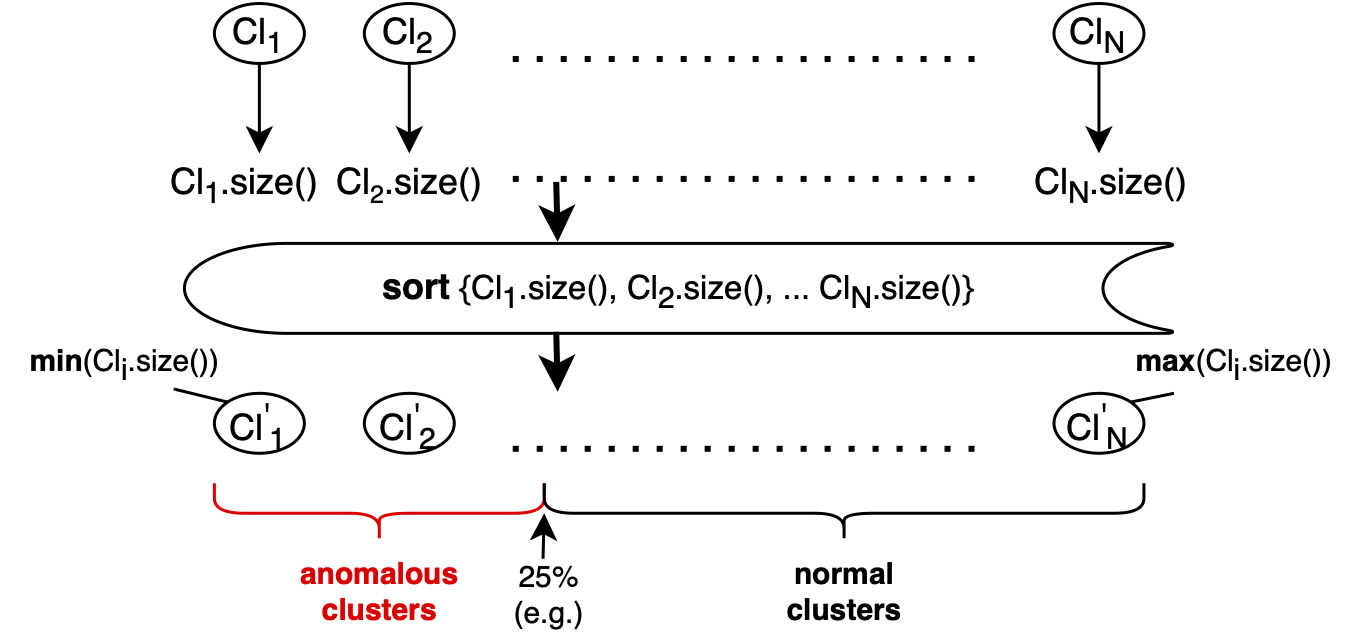
\includegraphics[width=0.8\textwidth]{images/cl-classif.png}
	\caption{Определение нормальных и аномальных кластеров}
	\label{fig:cl-classif}
\end{figure}

\subsection{Моделирование кластеров}

Чтобы более эффективно выполнить дальнейшую классификацию входной траектории, в выбранной в качестве основы работе было предложено создать модели кластеров (модели траекторий), классифицированных как нормальные или аномальные. Моделью кластера называется ее компактное представление. Модели нормальных кластеров можно рассматривать как шаблоны частых траекторий, поскольку они представляют собой весь кластер траекторий с максимальной точностью.

Существуют две основные концепции построения модели кластера \cite{article:surv_cl_models}:
\begin{itemize}
	\item выбор репрезентативной траектории из кластера. Такая траектория считается центром кластера. Самым простым способом обозначить репрезентативную траекторию является определение только ее центроида (центроид кластера, путь центроида). В качестве дополнения центроид может быть расширен определением диапазона, области пути центроида;
	\item определение модели на основании траекторий, относящихся к кластеру, с использованием вероятностных моделей, таких как Гауссовские наблюдательные эмиссионные HMM (Hidden Markov Model). Такой метод требует предварительной обработки траекторий и показвыает лучшие результаты на вероятностно моделируемых траекториях.
\end{itemize}

По сравнению со второй концепцией, выбор репрезентативной траектории для каждого кластера в качестве модели является более простым методом. Более того, он не требует, чтобы траектории имели одинаковое количество точек траектории \cite{inproceedings:7_related_work}.

Авторы \cite{inproceedings:7_related_work} предлагают легкий подход к моделированию кластера без какой-либо предварительной обработки траекторий: модель кластера - это траектория, наименее всего удаленная от других, в результате чего ее можно рассматривать как репрезентативный центр кластера. Это означает, что необходимо определить траекторию с минимальным средним расстоянием LCSS до других траекторий в этом кластере (\ref{eq:cm_traj}):

\begin{equation} \label{eq:cm_traj}
	CM(C) = \min\limits_{T \in C} \frac{1}{|C|} \sum_{T' \in C} D_{LCSS}(T, T')
\end{equation}

Рис. \ref{fig:cm-modeling} демонстрирует общий принцип выбора кластерной модели: в качестве кластерной модели выбирается таректория, максимально точно характеризующая группу траекторий.

\begin{figure}[!htb]
	\centering{}
	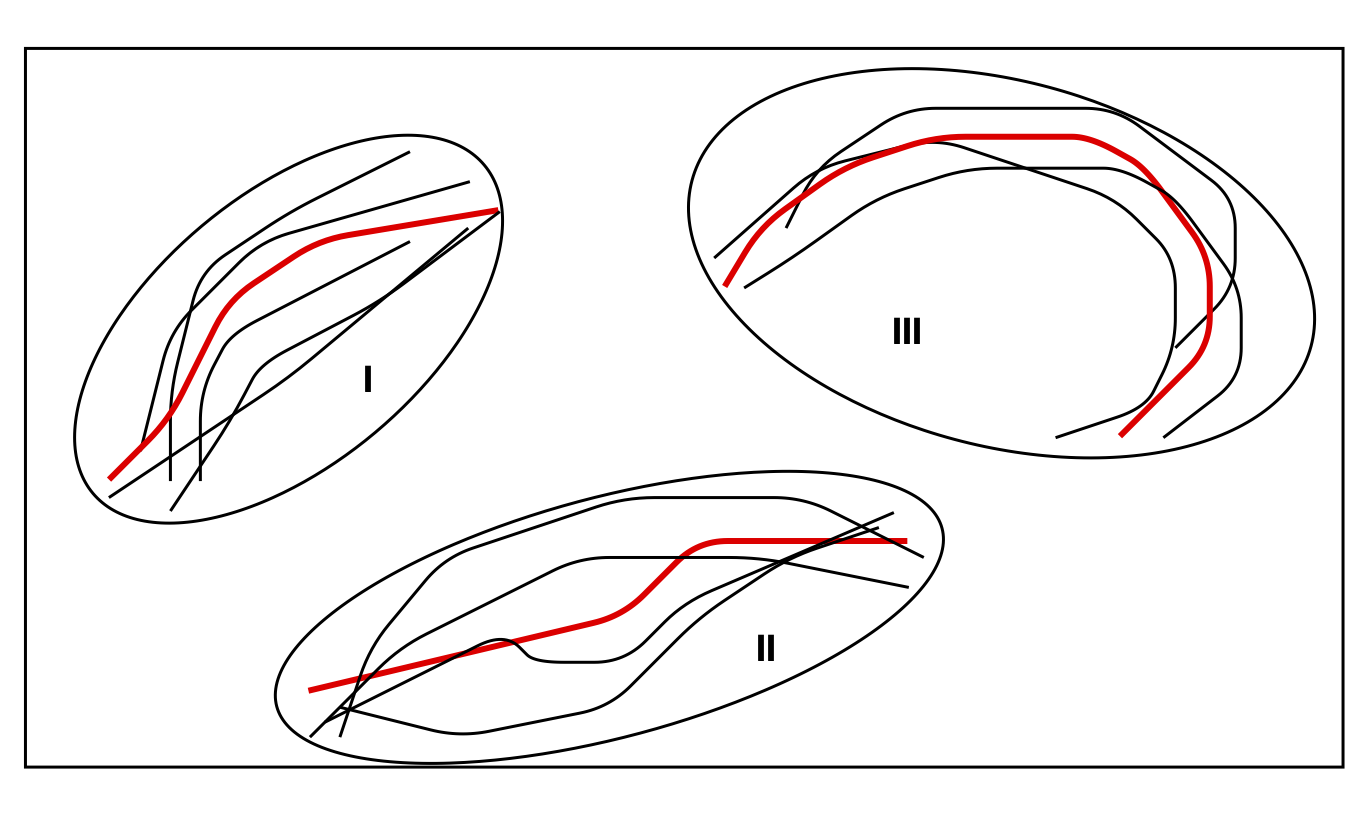
\includegraphics[width=0.7\textwidth]{images/cm-modeling.png}
	\caption{Выбор модели кластера}
	\label{fig:cm-modeling}
\end{figure}

Таким образом, моделирование кластеров реализуется для упрощения и ускорения этапа классификации, который в результате при использовании предложенного подхода выбора репрезентативной траектории для каждого кластера будет сводиться к подсчету расстояния между входной траекторией и каждой из кластерных моделей.

\section{Сравнение траекторий}

Для измерения схожести и расстояния между траекториями для выполнения кластеризации в этой работе будет использоваться LCSS расстояние. LCSS расстояние подразумевает вычисление самой длинной общей подпоследовательности между двумя входными траекториями с использованием двух значений параметров: $\delta$ и $\varepsilon$.

\subsection{LCSS метрика для измерения схожести траекторий}

Согласно методу LCSS, параметры $\delta$ и $\varepsilon$ являются постоянными и задаются заранее. Однако в текущем предлагаемом подходе для работы с неопределенностью данных о траектории, содержащих точки траектории, расположенные произвольным образом по отношению к камере, было решено реализовать адаптивность значений параметров. Будет исследована функциональная зависимость параметров от положения движущегося объекта на перекрестке относительно камеры.

При визуальном анализе траекторий, отображенных на исходных изображениях с камер, можно сделать несколько выводов: поскольку нижняя часть изображения представляет область, расположенную ближе к камере наблюдения, движущиеся объекты в верхней части изображения более отдалены от камеры, и в результате более плотно расположены относительно друг друга на изображении. $\varepsilon$ представляет собой пороговую величину, регулирующую пространственную удаленность точек траектории при подсчете расстояния между ними. Следовательно, он должен быть адаптирован к удаленности и уменьшаться по мере удаления точки траектории от камеры.

Описание алгоритма подсчета LCSS приведено в алг. \ref{algo:lcss-descr}.

\begin{algorithm}[!htb]
	\caption{Описание алгоритма LCSS метрики}
	\label{algo:lcss-descr}
	\SetAlgoLined
	\KwIn{First trajectory: $T_1$,\newline
			Second trajectory: $T_2$,\newline
			Temporal remoteness threshold: $\delta$,\newline
			Spatial remoteness threshold: $\varepsilon$
	}
	\KwOut{LCSS distance for two trajectories}
	\Begin{
		// Initialization \\
		- calculate length of $T_1$\;
		- calculate length of $T_2$\;
		// LCSS similarity calculation \newline	
		\eIf {$T_1$ or $T_2$ is empty}{
			return 0;	
		}{\eIf {difference between X-coordinates < $\varepsilon$ \newline
			AND difference between Y-coordinates < $\varepsilon$ \newline
			AND difference between trajectory lengths < $\delta$}{
				- increase LCSS by 1\;
				- call recursive for trajectories excluding last points\;
			}{
				- calculate LCSS for first trajectory and second trajectory 	excluding last point\;
				- calculate LCSS for first trajectory excluding last point and second trajectory\;
				- take maximum between these LCSS values\;
			}
		}
		// LCSS distance calculation \\
		LCSS distance = 1 - LCSS similarity / minimum(input lengths)
	}
\end{algorithm}

\subsection{Адаптивность параметров LCSS алгоритма}

Классический метод подсчета LCSS предполагает использование постоянных значений для параметров $\delta$ и $\varepsilon$ и не подразумевает их адаптивности. Тем не менее, одной из целей в этой работе является исследование возможности повышения точности результатов путем изучения функциональной зависимости между этими параметрами и удаленностью движущейся точки от камеры.

По причине того что камера расположена в фиксированном месте на перекрестке, возможны проблемы, связанные с перспективой. Из рис. \ref{fig:tr_p}, на котором изображено распределение исходных траекторий, видно, что при удалении от камеры, расположенной в нижней передней части изображения, траектории становятся более плотно расположенными относительно друг друга ( входные данные будут описаны и изображены в следующей главе). В случае константного значения $\varepsilon$, контролирующего допустимое пространственное отклонение между точками траектории при тестировании пространственного равенства точек траектории, точки траектории, расположенные далеко от камеры (то есть появляющиеся в верхней части изображений с камер и расположенные более плотно друг к другу), будут неправильно признаны похожими. Это может негативно повлиять на последующий анализ и исказить дальнейшие результаты кластеризации.

Следовательно, значение коэффициента $\varepsilon$ должно меняться в соответствии с расстоянием от местоположения камеры: $\varepsilon$ должен уменьшаться по мере удаления точки траектории от камеры и увеличиваться по мере приближения точки траектории к камере. Таким образом, можно предположить, что $\varepsilon$ и расстояние от камеры находятся в обратной зависимости, что означает, что в итоговой формуле расстояние от камеры должно присутствовать в знаменателе формулы с некоторым коэффициентом.

Подход к определению адаптивных параметров, рассмотренный в данной работе, описан в алг. \ref{algo:lcss-params-adapt} и изображен на рис. \ref{fig:adaptivity}.

\begin{algorithm}[!htb]
	\caption{Определение адаптивных параметров LCSS}
	\label{algo:lcss-params-adapt}
	\SetAlgoLined
	\KwIn{First trajectory point: $TP_1$,\newline
		Second trajectory point: $TP_2$
	}
	\KwOut{Adaptive $\varepsilon$ value for $TP_1$ and $TP_2$}
	\Begin{
		// Initialization \\
		- compute location of a camera point ($CP$)\;
		- compute Euclidean distance for two pairs $d_1$($TP_1$, $CP$) and $d_2$($TP_2$, $CP$)\;
		- compute corresponding $\varepsilon_1$ and $\varepsilon_2$ values\;
		- take the $\max(\varepsilon_1,\ \varepsilon_2)$ as a final $\varepsilon$ to compare $TP_1$ and $TP_2$.
	}
\end{algorithm}

\begin{figure}[!htb]
	\centering{}
	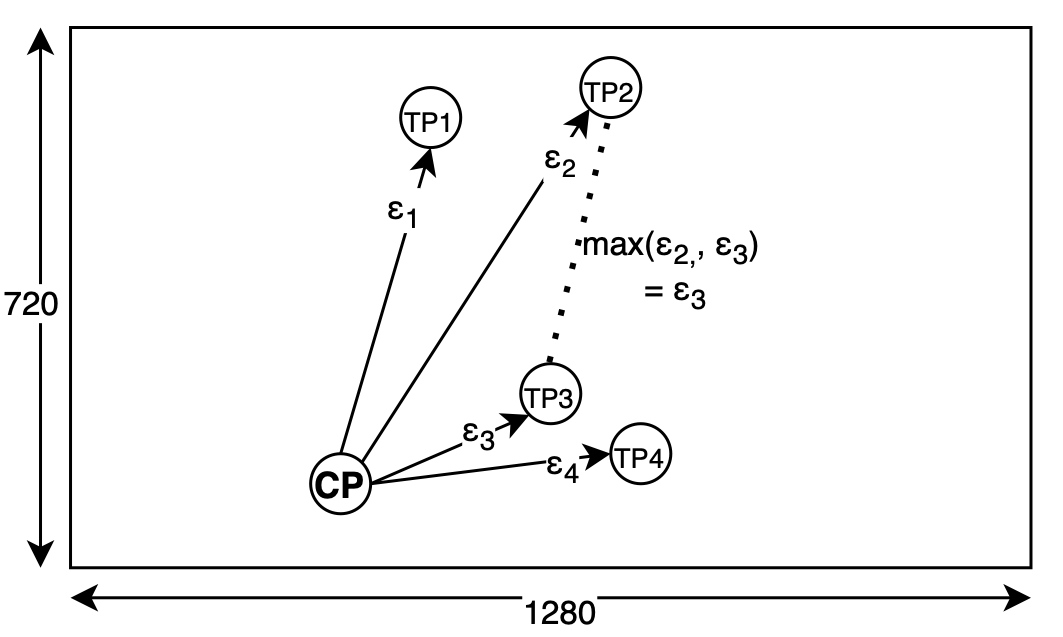
\includegraphics[width=0.7\textwidth]{images/adaptivity.png}
	\caption{Принцип выбора адаптивного значения $\varepsilon$}
	\label{fig:adaptivity}
\end{figure}

Чтобы оптимизировать подсчет расстояния от точки траектории до точки камеры и избежать его многократного пересчета во время работы алгоритма вычисления LCSS, это расстояние рассчитывается заранее и сохраняется для каждой точки траектории.

\section{Проверка достоверности кластеров}

Поскольку целью настоящей работы является поиск оптимальных значений адаптивных параметров для вычисления метрики сходства траекторий, необходимо проанализировать и сравнить полученные результаты после выполнения кластеризации.

Согласно \cite{online:dunn_cl_valid} метрики проверки достоверности результатов кластерного решения могут быть классифицированы следующим образом:
\begin{itemize}
	\item \textbf{Internal cluster validation} -- внутренняя метрика оценки кластеров. Результат кластеризации оценивается на основе кластеризованных входных данных. Он основан на внутренней информации и не содержит ссылок на внешнюю информацию.
	\item \textbf{External cluster validation} -- внешняя метрика оценки кластеров. Оценка результатов кластеризации выполняется в соответствии с известными извне результатами, например, данными метками класса. Такая проверка не подходит для неконтролируемой (unsupervised) кластеризации, поскольку в таком случае входные метки неизвестны.
	\item \textbf{Relative cluster validation} -- относительная метрика оценки кластеров. Оценка результатов кластеризации выполняется с помощью одного и того же алгоритма с использованием разных входных параметров, таких как количество кластеров и т.д..
\end{itemize}

В то же время кластеризация - это, прежде всего, метод бесконтрольного неконтролируемого извлечения данных, использующий входные данные, не содержащие меток данных. Это приводит к необходимости проверять итоговые кластеры неконтролируемым образом.

Одной из наиболее широко используемых и известных метрик для оценки алгоритмов кластеризации является индекс достоверности Данна (Dunn's Validity Index, DI), который был предложен Дж. К. Данном в 1974 году в \cite{article:dunn_orig}. Это внутренняя метрика оценки, предназначенная для идентификации компактных кластеров с небольшой дисперсией между элементами кластера, которые хорошо отделены друг от друга, то есть кластеры достаточно отдалены от окружающих кластеров по сравнению с межкластерной дисперсией \cite{online:hier_clust_r}. DI рассчитывается как отношение минимального межкластерного расстояния $d_{min}$ к максимальному внутрикластерному диаметру $d_{max}$, и для $k$ кластеров может быть определен следующим образом (\ref{eq:dunn-index}) \cite{article:quant_eval_perf_clust}:

\begin{equation} \label{eq:dunn-index}
	DI = \frac {d_{min}} {d_{max}} = \frac{\min\limits_{\substack{1 \leq i \leq k \\ i+1 \leq j \leq k}} dist(c_i, c_j)} {\max\limits_{1 \leq l \leq k} diam(c_l)}
\end{equation}

где минимальное межкластерное расстояние $d_{min}$ в соответствии с методом связи по минимальной ссылке сводится к подсчету минимального расстояния между двумя траекториями из разных кластеров. Максимальный внутрикластерный диаметр $d_{max}$, или самое большое внутрикластерное расстояние, предполагает вычисление диаметра кластера как расстояния между его двумя самыми дальними траекториями \cite{inproceedings:clust_ind}.

Пример определения DI для 3 кластеров приведен на рис. \ref{fig:di_sample}. Согласно этому примеру (\ref{eq:dunn-index-sample}) может быть переписан следующим образом:

\begin{equation} \label{eq:dunn-index-sample}
DI = \frac {d_{min}} {d_{max}} = \frac
	{\min ({dist_{min}}^1, {dist_{min}}^2, {dist_{min}}^3)}
	{\max ({diam_{max}}^1, {diam_{max}}^2, {diam_{max}}^3)}
\end{equation}

\begin{figure}[!htb]
	\centering{}
	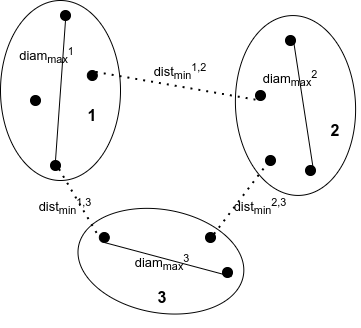
\includegraphics[width=0.5\textwidth]{images/di-sample.png}
	\caption{Объяснение индекса DI}
	\label{fig:di_sample}
\end{figure}

Более высокие значения DI указывают на лучшие результаты кластеризации. Траектории, расположенные далеко друг от друга внутри одного кластера, должны отличаться от траекторий, относящихся к другим кластерам. Близкие к 1 значения DI означают, что минимальные расстояния до траекторий из разных кластеров остаются больше, чем расстояние до самых дальних траекторий внутри одного кластера. Однако вычислительная стоимость DI сильно зависит от данных: вычислительная сложность увеличивается с ростом количества кластеров и размерности данных \cite{online:dunn_cl_valid}.

\section{Аппроксимация траекторий}

Несмотря на то что метрика подобия LCSS работает с траекториями произвольных длин и по умолчанию не требует предварительной обработки траекторий, подсчет LCSS метрики становится чрезвычайно вычислительно сложным и времязатратным с ростом длины траектории в результате рекурсивности. По этой причине в текущей работе было решено уменьшить размер траекторий путем аппроксимации исходных траекторий. Это приводит к потере точности, но позволяет получить приемлемые результаты за адекватное количество времени.

Концепция подбора аппроксимирующей кривой функции - это один из стандартных подходов для выполнения аппроксимации \cite{article:behav_form_extr}. Основная задача - найти подходящее соотношение или закон, возможно существующий между входными (независимыми) и выходными (зависимыми) переменными для заданного набора входных данных наблюдаемых значений. И подбор кривой - это процесс выражения связи между переменными в терминах алгебраических уравнений. Основная цель подбора кривой - найти параметры для модели (уравнения или функции), подходящей для экспериментальных данных.

\subsection{Регрессионный анализ}

Одним из наиболее широко используемых подходов, основанных на концепции подбора кривой, является регрессионный анализ, который также рассматривается как форма подхода прогнозирующего моделирования и, согласно традиционному определению, изучает взаимосвязь между зависимой переменной (результатом) $Y$ и одним или более независимыми переменными $X$ и, как правило, находит тренды в данных. Другими словами, он предполагает «использование отношения между переменными для подбора линии наилучшего соответствия или уравнения регрессии, которое можно использовать для прогнозирования» \cite{online:intro_lr_pr}.

С целью упростить процедуру подбора аппроксимирующей функции обычно предполагается, что независимые переменные $X$ измеряются без ошибок, в то время как значения зависимых переменных $Y$ измеряются с некоторой случайной ошибкой. Для данных с небольшим отношением ошибки измерения в независимой переменной к диапазону значений этой переменной можно правомерно использовать регрессионный анализ по методу наименьших квадратов \cite{article:behav_form_extr}.

Регрессия может быть линейной или полиномиальной (нелинейной, криволинейной) в зависимости от функции, которая аппроксимирует данные: линейная регрессия применима к отношениям, аппроксимируемым прямой линией, тогда как криволинейная регрессия относится к отношениям,  аппроксимируемым кривой. Благодаря более широкому диапазону функций, с которыми может работать полиномиальная регрессия, она обеспечивает лучшее приближение входных отношений по сравнению с линейной регрессией \cite{online:intro_lr_pr}. Даже если невозможно заранее определить тип функции для аппроксимации, чтобы получить наивысшую точность результатов, может оказаться полезным визуализация и анализ отображения исходных данных для нахождения какого-либо поведенческого паттерна, такого как линейная, квадратичная или зависимость более высокого порядка \cite{article:behav_form_extr}.

\subsection{Полиномиальная регрессия}

Визуализация исходных данных траекторий представлена на рис. \ref{fig:tr_p}. Как видно из рисунка, ни линейные функции, ни функции $2$-го порядка не могут соответствовать данным должным образом из-за сложности форм траектории. По этой причине было решено сосредоточиться на приближении с использованием полиномиальной регрессии высшего порядка. Оценка полиномиальной регрессии с различными степенями будет приведена далее, и последующее обсуждение и реализация будут направлены на то, чтобы найти подходящее полиномиальное уравнение $n$-го порядка со значениями параметров для представления каждой входной траектории в качестве «функции траектории». Поскольку данные траектории представлены двумерными пространственными данными вместе с временными данными, и необходимо аппроксимировать пространственную информацию, $x$- и $y$ -координаты будут рассматриваться как зависимые переменные, а $time$ будет использоваться как независимая переменная. Следовательно, полиномиальная регрессия будет выполняться дважды с двумя выходными полиномиальными функциями, представляющими $x(t)$ и $y(t)$ для каждой из входных траекторий $T$:

\begin{equation}\label{eq:regr-func}
	\forall\ T = [\ldots (x_i, y_i, t_i) \ldots] = > T(t) = 
		\begin{cases}
			x = x(t) \\
			y = y(t) \\
		\end{cases}
\end{equation}

Таким образом, траектории будут преобразованы из формата списка точек траекторий в уравнения (функции времени), определенные в геометрическом пространстве, которые могут с высокой точностью представлять все исходные траектории. Выбор ключевых точек репрезентативного полинома может уменьшить размер траектории, тем самым сокращая итоговые эксплуатационные затраты и вычислительную сложность LCSS. Кроме того, математические уравнения способны хранить информацию в плотной форме, и, помимо других преимуществ, такое сокращение данных приводит к уменьшению занимаемого пространства и повышению эффективности хранения \cite{article:behav_form_extr}. Также так называемые встроенные «функции траектории» могут обеспечивать интерполяцию и позволяют определять пропущенные, потерянные точки траекторий.
